%%%%%%%%%%%%%%%%%%%%%%%%%%%%%%%%%%%%%%%%%%%%%%%%%%%%%%%%%%%%%%%%%%%%%%%%%%%%%%%%

\documentclass[a4paper, 10pt, conference]{ieeeconf}      % Use this line for a4
\usepackage[]{graphicx}  
\usepackage{multirow}
\usepackage{tabularx}
\overrideIEEEmargins
% See the \addtolength command later in the file to balance the column lengths
% on the last page of the document

% The following packages can be found on http:\\www.ctan.org
\usepackage{xcolor} % for pdf, bitmapped graphics files
\usepackage[dvipsnames]{xcolor}
\pagenumbering{arabic}
\title{\LARGE \bf
Customer Churn Analysis}

\setcounter{page}{1}

\author{Aishwarya Paruchuri, Archita Chakraborty, Manjushree Rajanna, Rohit Chandra\\San Jose State University\\ November 2021% <-this % stops a space
}

\date{November 2021}

\begin{document}



\maketitle
\thispagestyle{empty}
\pagestyle{empty}


%%%%%%%%%%%%%%%%%%%%%%%%%%%%%%%%%%%%%%%%%%%%%%%%%%%%%%%%%%%%%%%%%%%%%%%%%%%%%%%%
\\\
\begin{abstract}
\\
To survive in today’s telecommunication business it is important to identify customers who are not hesitant to move towards a competitor. As a result, predicting customer attrition has become a critical concern in the industry. The capacity of a data-driven churn prediction system to be comprehensive and actionable is dependent on the effective extraction of hidden patterns from the data. In this paper, customer information was retrieved using data from an Iranian mobile company, and the key problem was dealing with data imbalance, which was addressed using techniques like SMOTE and undersampling.The results were then compared between balanced (SMOTE, undersampling) data and imbalanced data with respect to different classifiers. The results showed a high precision (96.5\%) and recall (97.23\%) on SMOTE imputed data. After analysing the data, factors which were affecting the churn analysis were identified and measures to mitigate their customer churn rate were proposed.


\end{abstract}


%%%%%%%%%%%%%%%%%%%%%%%%%%%%%%%%%%%%%%%%%%%%%%%%%%%%%%%%%%%%%%%%%%%%%%%%%%%%%%%%
\\\
\section{\textbf{Introduction}}

The mobile services market is growing significantly and sustainably, not only due to the size of the market, but also due to the increasing variety of services offered and fierce competition in the telecommunication industry. Regardless of the earliest stages of this industry, the method of contest has moved from procuring new endorsers to holding existing customers. This has been accomplished by participating in showcasing endeavors and by luring customers from rival organizations.
\\
\\Based on a Jan 2020 article, Accenture reports that 77\% of consumers now retract their loyalty more quickly than they did three years ago and industry must therefore work harder than ever to retain their customer bases. Acquisition costs far outweigh those of keeping current customers, further motivating companies to implement innovative strategies to boost customer retention in the telecom industry. This is further underscored by research from Bain & Company suggesting that a mere 5\% increase in a company’s retention rate can increase profits by 25\% to 95\%.[5]Hence, financially, it makes more sense for an organization to focus on retaining its existing customers. As a result, churn management is a major area of focus.
\\
\\In this study to predict the customer churn rate, the imbalanced data is treated with different techniques such as SMOTE and under sampling and then the data is fed to different classifiers. So, for the imbalanced dataset, we chose the xgboost classifier, which is robust to imbalanced data, and for the balanced dataset, we tried many other classifiers such as random forest, logistic regression, and others, and found that Naive Bayes classifier, decision tree, and support vector classifier gave better results. The results are then compared based on different  performance metrics such as Precision, Recall, F1 score and RoC value. 

\subsection{\textbf{Dataset}}
\\The data set has been collected from an Iranian telecommunication company’s database over a period of 12 months. It contains 3150 customer data with the following features:
\\
\\\
\begin{tabularx}{0.45\textwidth} { 
  | >{\centering}X 
  | >{\centering}X 
  | >{\raggedright\arraybackslash}X | }
 \hline
 \textbf{Feature name} &\textbf {Type} & \textbf {Description} \\
 \hline
Call Failures & Numerical & Number of call failures \\
 \hline
Complains & Categorical & (0: No complaint,1: complaint) \\ 
\hline
Charge Amount & Categorical & 0: lowest amount, 9: highest amount \\
\hline
Seconds of Use & Numerical & total seconds of calls \\
\hline
Frequency of use & Numerical & total number of calls \\
\hline
Frequency of SMS & Numerical & total number of text messages \\
\hline
Distinct Called Numbers & Numerical & total number of distinct phone calls \\
\hline
Tariff Plan & Categorical & binary (1: Pay as you go, 2: contractual) \\
\hline
AgeGroup & Categorical & 1: younger age, 5: older age \\
\hline
Status & Categorical & binary (1: active, 2: non-active) \\
\hline
Customer Value & Numerical & The calculated value of customer \\
\hline
Subscription length & Numerical &  Total months of subscription \\
\hline
Churn & Categorical & binary (1: churn, 0: non-churn) - Class label \\
\hline
\end{tabularx}
% \begin{figure}[htp] 

\\\textbf{Note:} The output feature - "churn" has  495 records which belongs to the churned class and 2645 records belong to the non-churned class. This shows that the data is highly imbalanced.
\\\
% \subsection{\textbf{Association Analysis}}
% \\\
% \\Multiple factors can affect customer churn(Fig. 1).
% \\\
% \\1. {Customer dissatisfaction}: 
% Customer complaints and Service failure rates are positively associated and length of customer association is negatively associated with customer churn probability. 
% \\\
% \\2. {Level of service usage}: 
% Number of calls, Minutes of monthly use and Number of distinct calls are negatively associated with customer churn probability. 
% \\\
% \\3. {Switching costs}: 
% Type of service is positively associated with the probability of subscriber churn.
% \\\
% \\4. {Customer demographic variable}: 
% Customer age is positively associated with customer churn probability.
% \\\
% % \usepackage{graphicx}
% \begin{figure}[htp]
%     \centering
%     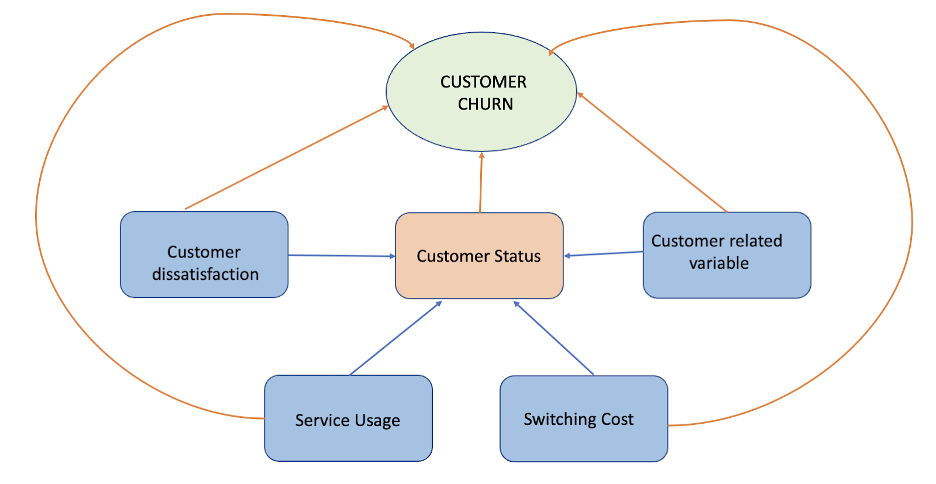
\includegraphics[scale= .55]{Images/AssociationAnalysis.png}
%     \caption{Association Analysis}
%     \label{fig:AssociationAnalysis}
% \end{figure}
% \\
\subsection{\textbf{ Exploratory Data Analysis}}
\\\
\\\
\textbf{1. Data Preprocessing}

\\It's a data mining approach for converting raw data into a usable and efficient format to derive meaningful information out of it.
\\\
\\
\textbf{Steps Involved in Data Preprocessing:} 
\\
\\\
\textbf{(A) Data Cleaning} 
\\There may be various useless and missing elements in the raw data. Data cleaning is used to deal with this aspect. It entails dealing with missing data and noisy data.
% \\\
% Handling Missing Data: This situation arises when some data is missing in the data.
% \\\
\\ Method used to find the null values: Missingno()
\\
\\
\begin{figure}[htp]
    \centering
    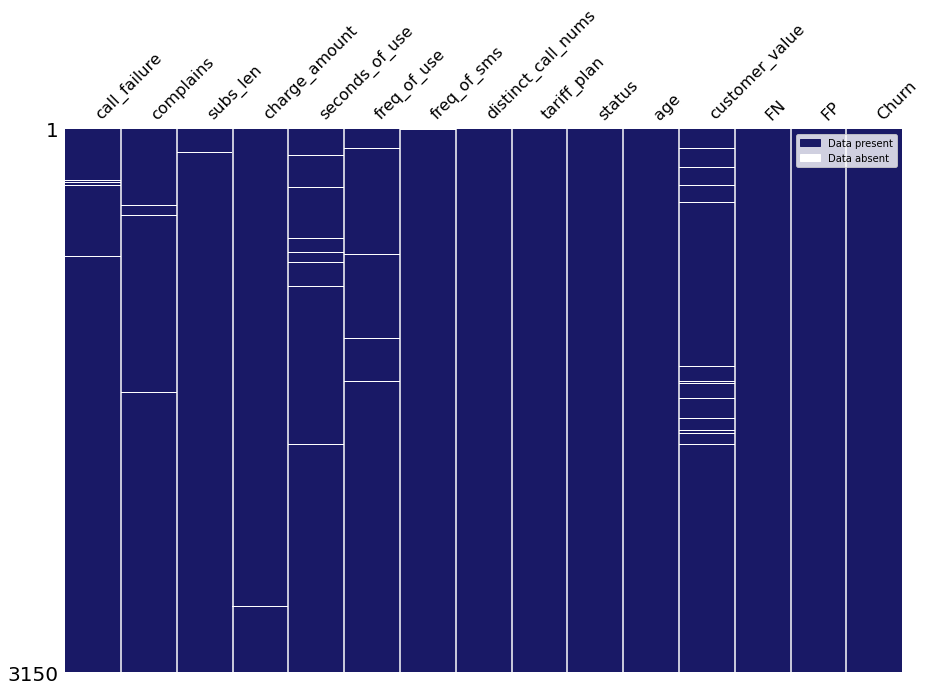
\includegraphics[width=8cm,height=6cm]{Images/missing_Plot.png}
    \caption{Missingo Matrix Plot}
    \label{fig:MissingnoBarPlot}
\end{figure}
\\\
\\
\textit{\textbf{Observation:} Missing values are shown by white striped lines in each column. The columns such as, call failure, complaints, subscription length, charge amount, seconds of use, frequency of use, and customer value have missing values that must be cleaned.}
\\\
\\\
\textbf{Techniques used to handle null values in the data:}
\\
\\\textbf{i) Median:} Few attributes, such as {secondsOfUse} and {customerValue}, have outliers. We impute median value in place of null values for these columns because mean is prone to outliers.
\\\
\\\textbf{ii) Mean :} We impute mean values in place of  null values for the remaining features that don't have outliers.
\\\
\\\
\textbf{(B) Outlier Detection}
\\\
\\Outliers are extreme values that deviate from other observations on data , they may indicate a variability in a measurement, experimental errors or a novelty. In other words, an outlier is an observation that diverges from an overall pattern on a sample.

\begin{figure}[htp]
    \centering
    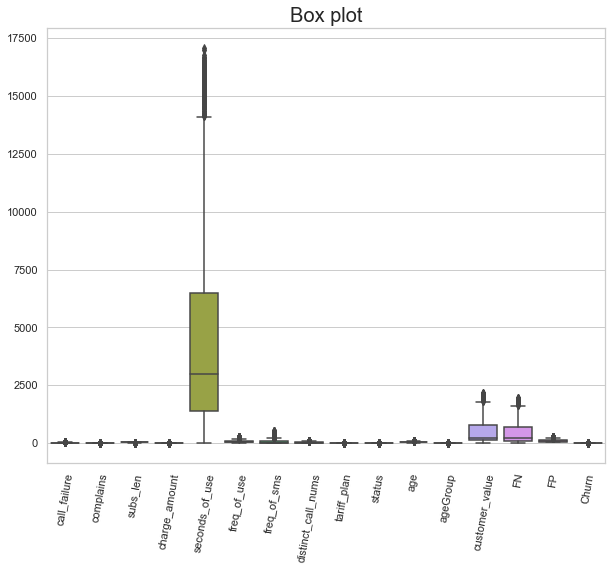
\includegraphics[width=8cm,height=6cm]{Images/boxplot.png}
    \caption{Null Values in each column of the data set}
    \label{fig:boxplot}
\end{figure}
\\\
\\\
\textit{\textbf{Observation:} As we can see in Fig.2, there are outliers in our data set, especially seconds of use feature has the most outliers.}
\\\
\\\
\textbf{Methods used to treat Outliers:}
\\i) Drop the outliers
\\ii) Replace with median or a constant value

\\\
\\\textbf{2. Feature Scaling}
\\This step is conducted to convert the data into a format that can be used in the mining process. Some of the classification models are based on probability, so we have scaled the data using MinMaxScalar() which transforms the values between 0 to 1 instead of StandardScalar() which transforms the data between -1 to 1.
 

 
\\\
\\\textbf{3. Data Visualizations}
\\\
\\The graphical depiction of information and data is known as data visualisation. Data visualisation tools make it easy to examine and comprehend trends, outliers, and patterns in data by employing visual elements like charts, graphs, and maps.
\\\
\\\
\\\textbf{Distribution of the output feature - "Churn":}
\\
\begin{figure}[htp]
    \centering
    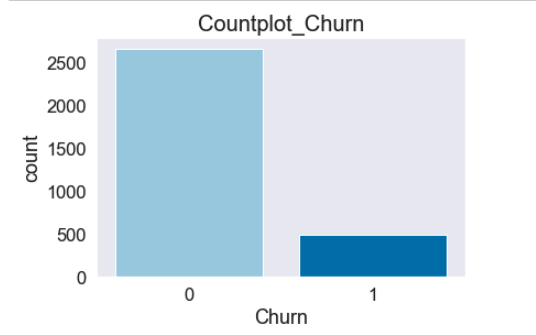
\includegraphics[width=6cm,height=5cm]{Images/churn_destribution_bar.png}
    \caption{Distribution of Churn}
\end{figure}
\\\
\textit{\textbf{Observation for fig 3:} For the predictor feature, we observe that there are 84.29 percent non-churn customers and 15.71 percent churn customers in total, indicating a data imbalance.}
\\\
\\
\\\textbf{Distribution of all the categorical features:}
\begin{figure}[htp]
    \centering
    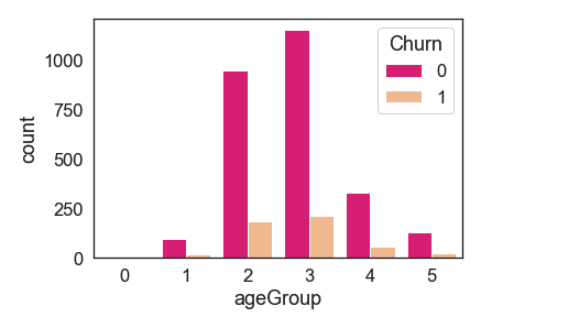
\includegraphics[width=7cm,height=5cm]{Images/ageGroup.png}
    \caption{Frequency Distribution of Age Group feature}
    \label{fig:frequencyDistribution}
\end{figure}
\\\
\\\textit{\textbf{Observation:} We notice that most number of the customers which are likely to churn are between the ages of 30-40 followed by age group 20-30 and over 40 years}

\begin{figure}[htp]
    \centering
    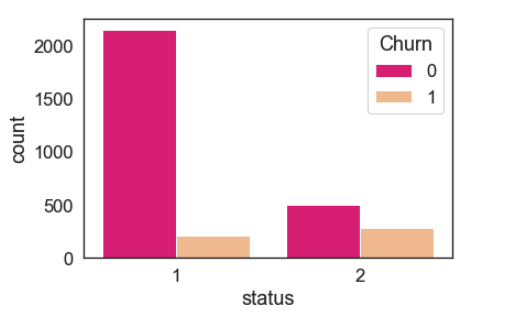
\includegraphics[width=8cm,height=5cm]{Images/Status.png}
    \caption{Frequency Distribution of Status feature}
    \label{fig:frequencyDistribution}
\end{figure}
\\\
\\\textit{\textbf{Observation:} We observe that the inactive customers are more likely to churn when compared to the customers which are actively using the service or subscription}
\\\
\\\
\begin{figure}[htp]
    \centering
    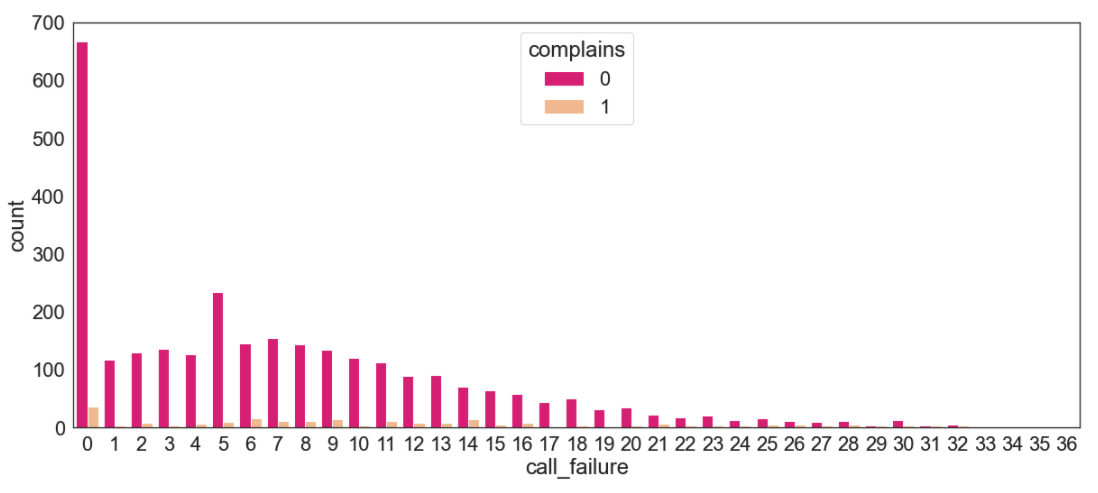
\includegraphics[width=8cm,height=5cm]{Images/call_failure.png}
    \caption{Frequency Distribution of Complaints feature}
    \label{fig:frequencyDistribution}
\end{figure}

 \\\textit{\textbf{Observation:} From the fig. 6 we observe that there's a higher percentage of consumers have no call failures and thus no complaints.}
 \\
 \\\
\textbf{Distribution of some of the numerical features:}

\begin{figure}[htp]
    \centering
    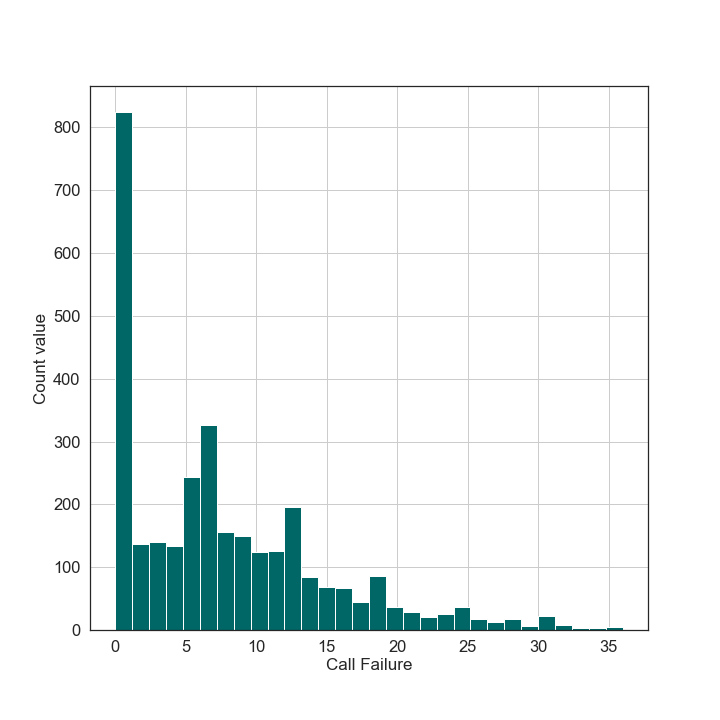
\includegraphics[width=8cm,height=5cm]{Images/frequency_distribution_call_failure.png}
    \caption{Distribution of call failure}
    \label{fig: Distribution of call failure}
\end{figure}
 \\\textit{\textbf{Observation:} We notice that approximately 2300 customers had call failures which states that this factor may be decisive in calculating the customer churn rate}
\begin{figure}[htp]
    \centering
    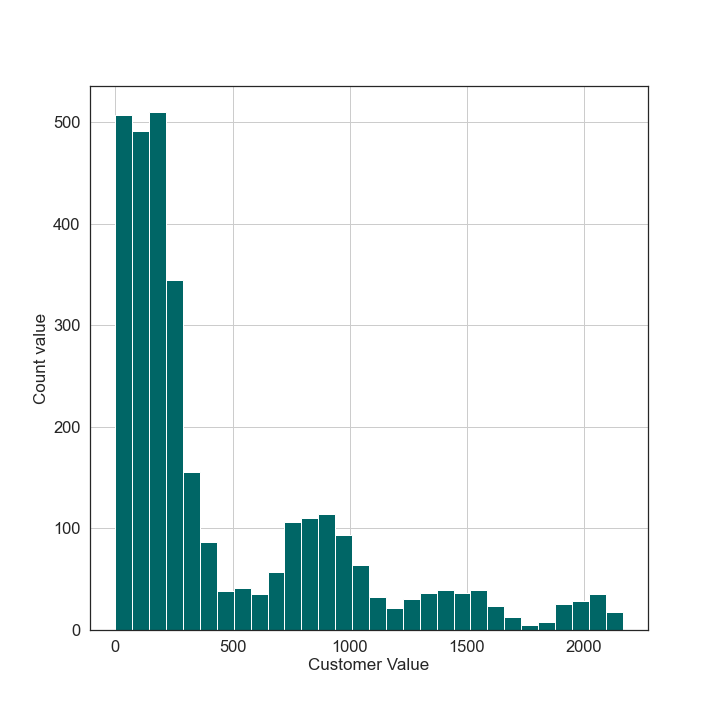
\includegraphics[width=8cm,height=5cm]{Images/frequency_distribution_customer_value.png}
    \caption{Distribution of customer value}
    \label{fig: Distribution of customer value}
\end{figure}
\\\
\\\textit{\textbf{Observation:} We notice that customer value is right skewed. Many customers have less customer value which implies that most of the customers are new and there might be a high risk of attrition with these customers }

\begin{figure}[htp]
    \centering
    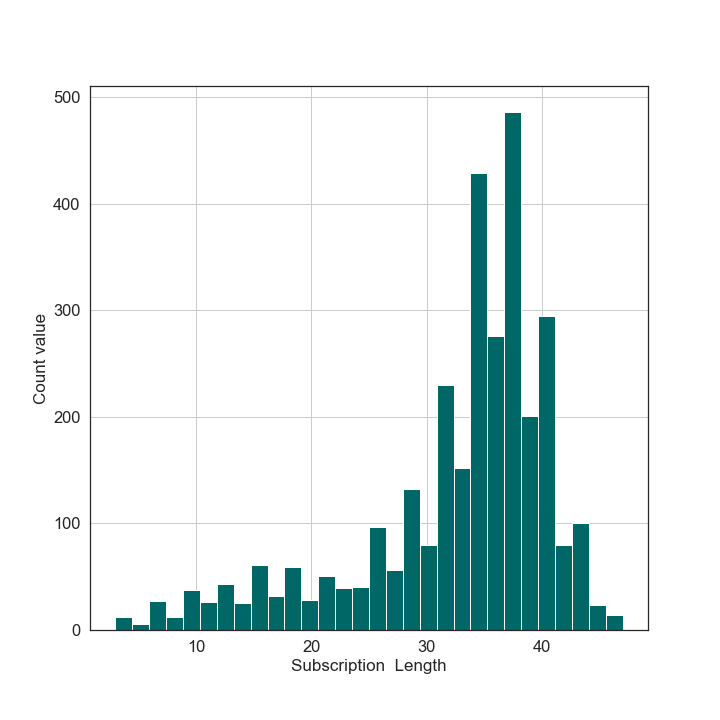
\includegraphics[width=8cm,height=5cm]{Images/frequency_distribution_Subscription_Length.png}
    \caption{Distribution of Subscription Length}
    \label{fig: Distribution of Subscription Length}
\end{figure}

\\\textit{\textbf{Observation:} Above plot shows that larger number of customers had a longer subscription length.}
\\
\\
\textbf{4. Feature Engineering}
\\\
\\It involves deriving new features based on the existing features in the data set. In the data set, We have identified Age feature and performed feature engineering on it to create a new feature called AgeGroup to combine different age values in
five different age intervals. The following table shows the age intervals:

\\
\begin{figure}[htp]
    \centering
    \includegraphics[width=5cm,height=4cm]{Images/agegrouptable.png}
    \caption{Table: Age Group}
    \label{fig:agegrouptable}
\end{figure}

\\\
\begin{figure}[htp]
    \centering
    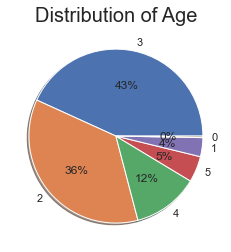
\includegraphics[width=5cm,height=5.5cm]{Images/distributionOfAge.png}
    \caption{Pie Chart displaying the age distribution of customers}
    \label{fig:distributionOfAge}
\end{figure}
\\\
\\\
\textit{Observation- As we can see from the pie chart, most of the customers belong to the age group 30-45.}

\\\
\\\textbf{5. Correlation analysis}

\begin{figure}[htp]
    \centering
    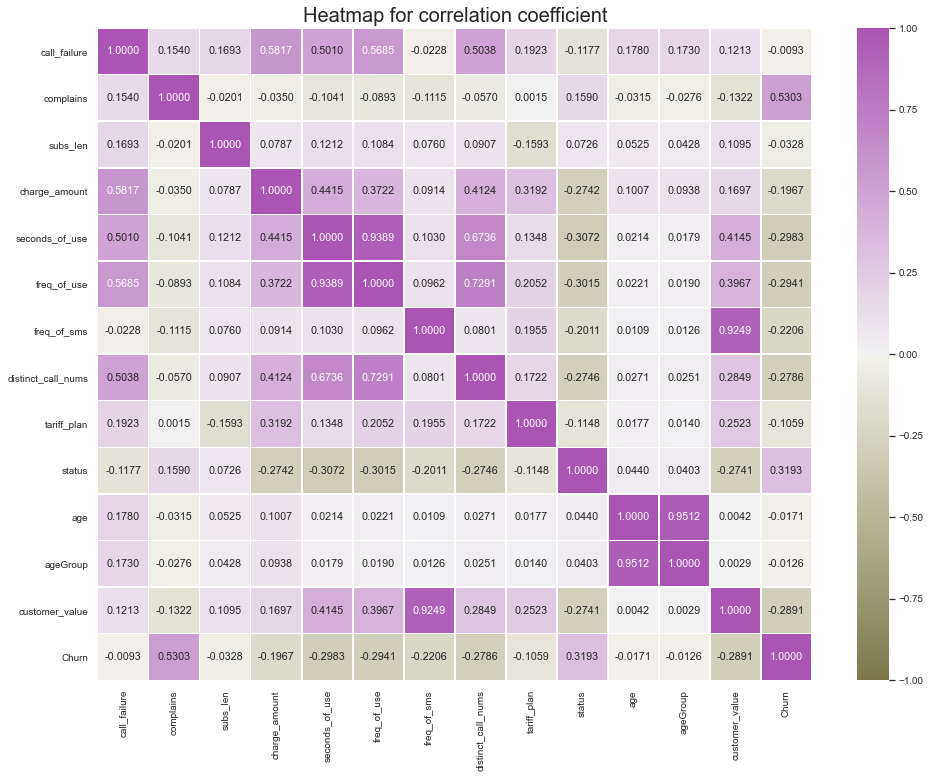
\includegraphics[width=8cm,height=6cm]{Images/heatmap.png}
    \caption{Heatmap for correlation coefficient}
    \label{fig:heatmap}
\end{figure}
\\\
\\From Fig.12 :
\\\textit{a: We observe a  positive correlation between freq of use and distinct call numbers. The correlation coefficient value is 0.9389.
\\b: We observe a  positive correlation between charge amount and call failure. The correlation coefficient value is 0.5817.
\\c: We observe a  positive correlation between freq of use and customer value. The correlation coefficient value is 0.9249.
\\d: We observe very less correlation between call failure and churn. The correlation coefficient value is -0.0093.}
\\\

\\\textbf{6. Feature Selection}
\\
\\We used SelectKBest feature selection technique to select the top features to train different multi-classification model. We can visualize with the help of horizontal bar plot shown below.
\begin{figure}[htp]
    \centering
    
\includegraphics[width=7cm,height=5cm]{Images/featureImportance.png}
    \caption{Churn vs all features}
    \label{fig:featureImportance}
\end{figure}

\\\textit{\textbf{Observation:} From the graph we observe that status and complain are influential features for this dataset.}

\\\
\section{\textbf{METHODS}}
As the data is highly imbalanced, we used Synthetic Minority Oversampling Technique(SMOTE), which involves duplicating samples in the minority class and Under Sampling Majority data set technique(UnderSampling), which randomly adds more minority observations by replication.
All our analysis is done with imbalanced data, SMOTE generated data and under-sampling generated data. While training models on these datasets, we performed hyper-parameter tuning using GridSearchCV, which loops over predefined hyper-parameters and fits the model to the training data using best parameter values obtained.
So, for the imbalanced dataset, we chose the xgboost classifier, which is robust to imbalanced data, and for the balanced dataset, we tried many other classifiers such as random forest, logistic regression, and others, and found that Naive Bayes classifier, decision tree, and support vector classifier gave better results.
Therefore, we considered following models to analyse the data:
\\\
\\\textbf{1) XGBoost Classifier:}
XGBoost is a decision-tree-based ensemble Machine Learning algorithm that uses a gradient boosting framework. The goal is to improve weak learners by using a gradient descent approach to minimise errors. When compared to other algorithms, it is thought to be exceptionally efficient and quick. We used this technique as it performs well with  unbalanced classification datasets, it does provide a way to modify the training process to pay greater attention to minority class in datasets with a skewed class distribution. Which is required in our case, as our data suffers from severe data imbalance.
XGBoost classifier yields following results:

\\\
\begin{figure}[htp]
    \centering
    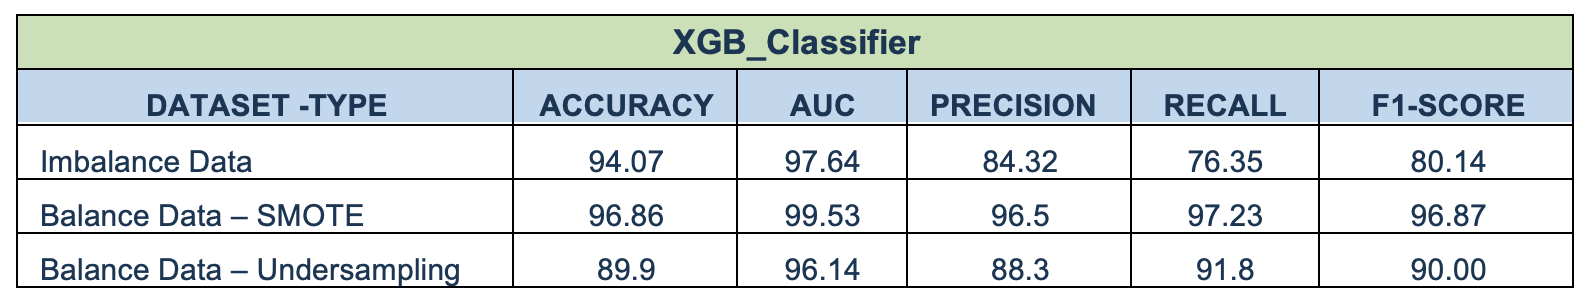
\includegraphics[width=8cm,height=2cm]{Images/xgbclassifier.png}
    \caption{XGB Classifier Results}
    \label{fig:xgbclassifier}
\end{figure}
\\\
\\\textbf{2) Naive Bayes Classifier:} The Bayes Theorem-based probabilistic machine learning method Naive Bayes(NB) is employed in a wide range of categorization problems.

\\\
\\\textbf{2a) Gaussian Naive Bayes Classifier:} It is a naive bayes algorithm that is unique. When the features have continuous values, it's employed particularly. It's also expected that all of the characteristics have a Gaussian distribution, or a normal distribution.
Gaussian Naive Bayes Classifier yields following results:

\begin{figure}[htp]
    \centering
    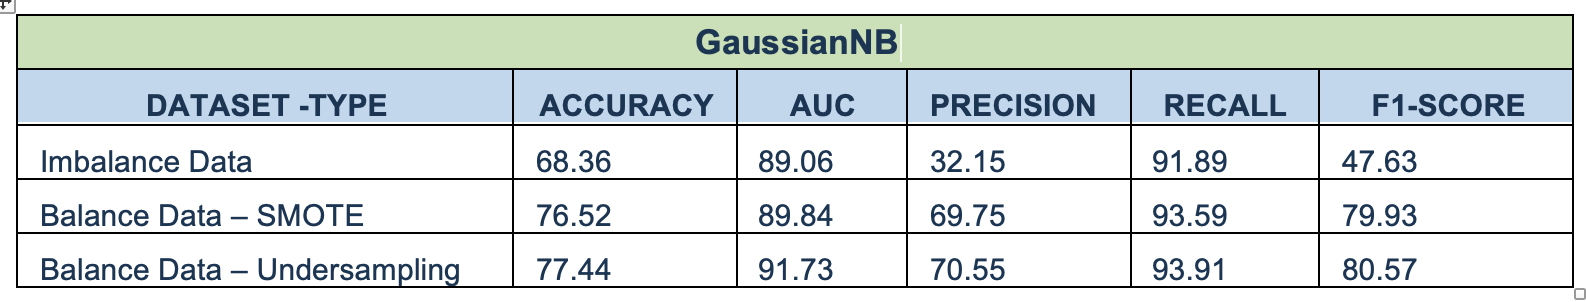
\includegraphics[width=8cm,height=2cm]{Images/GaussianNB.png}
    \caption{GaussianNB Classifier Results}
    \label{fig:GaussianNB}
\end{figure}
\\\
\\\textbf{2b) Multinomial Naive Bayes Classifier:} It is suitable for classification with discrete features (e.g., word counts for text classification). The multinomial distribution normally requires integer feature counts. 
Multinomial Naive Bayes Classifier yields following results:

\begin{figure}[htp]
    \centering
    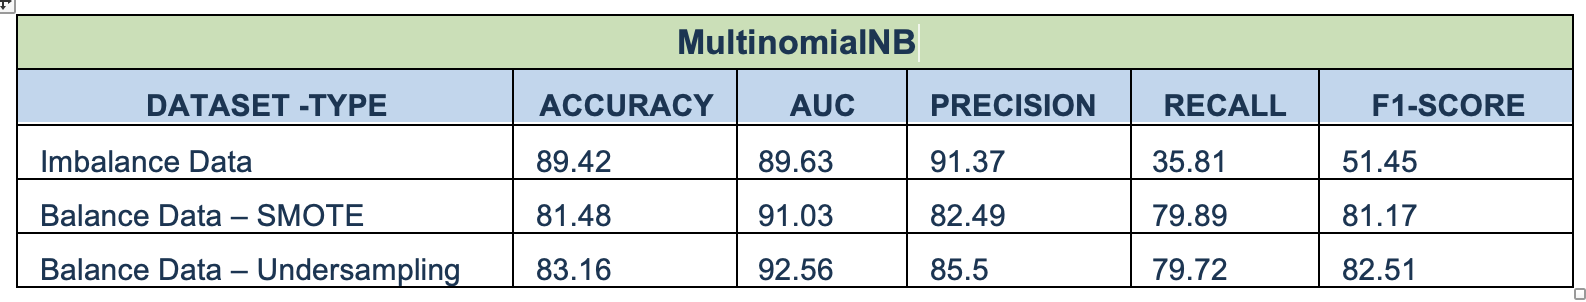
\includegraphics[width=8cm,height=2cm]{Images/MultinomialNB.png}
    \caption{Multinomial Classifier Results}
    \label{fig:MultinomialNB}
\end{figure}
\\\
\\\textbf{2c) Complement Naive Bayes Classifier:} It is well-suited to dealing with unbalanced data sets. Instead of calculating the probability of an item belonging to a certain class, we calculate the probability of the item belonging to all classes in complement Naive Bayes.
Complement Naive Bayes Classifier yields following results:

\begin{figure}[htp]
    \centering
    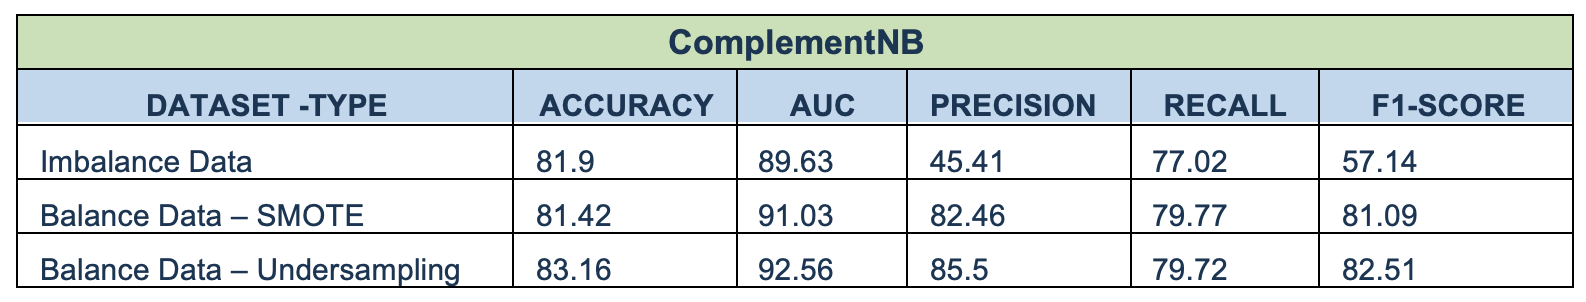
\includegraphics[width=8cm,height=2cm]{Images/ComplementNB.png}
    \caption{ComplementNB Classifier Results}
    \label{fig:ComplementNB}
\end{figure}
\\\
\\\
\\\textbf{3) Support Vector Classifier(SVC):} It is a linear model that can be used to solve classification and regression problems. It can solve both linear and nonlinear problems.The algorithm generates a line or hyper-plane that divides the data into categories.
 Support Vector Classifier yields following results:
\\\
\begin{figure}[htp]
    \centering
    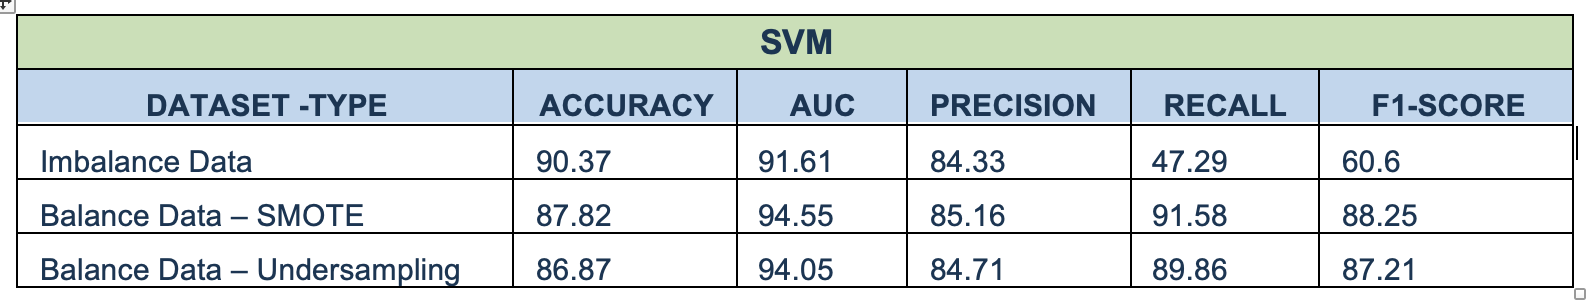
\includegraphics[width=8cm,height=2cm]{Images/svm.png}
    \caption{SVM Classifier Results}
    \label{fig:svm}
\end{figure}
\\\
\\\textbf{4) Decision Tree:} It is supervised machine learning that categorises or predicts outcomes based on the answers to a previous set of questions.
Decision Tree yields following results:

\\\
\begin{figure}[htp]
    \centering
    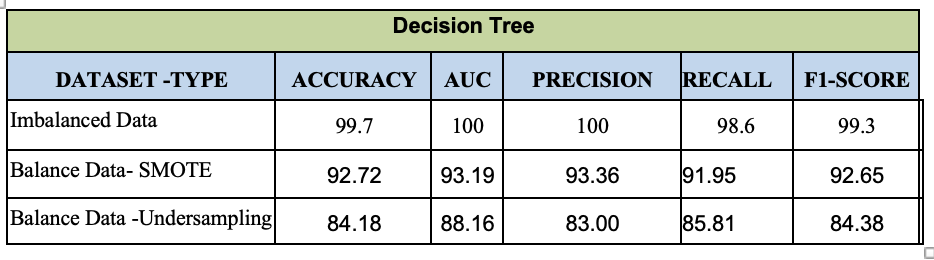
\includegraphics[width=8cm,height=2.5cm]{Images/decisionTree.png}
    \caption{Decision Tree Classifier Results}
    \label{fig:decisionTree}
\end{figure}
\\
\section{\textbf{COMPARISIONS}}
\\\
\\\subsection{\textbf{Performance Metrics}}
\\\
\\1. Precision- The number of positive class predictions that actually belong to the positive class is measured by precision.
\\\
\\2. Recall- The number of positive class predictions made out of all positive examples in the dataset is measured by recall.
\\\
\\3. F1-Score- F1-Score generates a single score that accounts for both precision and recall concerns in a single number.
\\\
\\4. Accuracy- It's the proportion of correct predictions to total input samples. It only works if each class has an equal amount of samples. 
\\\
\\5. AUC - The Area Under the Curve (AUC) is a  curve that measures a classifier's ability to distinguish between classes. The greater the AUC, the better.
\\\
\\Note: Since our data is class imbalanced, we majorly rely on F1-Score, Recall and Precision.
\\\
\subsection{\textbf{Comparison}}
\\\
\\
Among all the models trained on imbalanced data, XGBoost is the winner as XGBoost can offer better performance on binary classification problems with a severe class imbalance.The model performed better with good precision(84.32 percent) as well as recall score(76.35 percent). The Fig.18 depicts the high AUC percentage(98 percentage) of XGBoost Classifier wrt other models. 
\\\
\\\
\\\
\begin{figure}[htp]
    \centering
    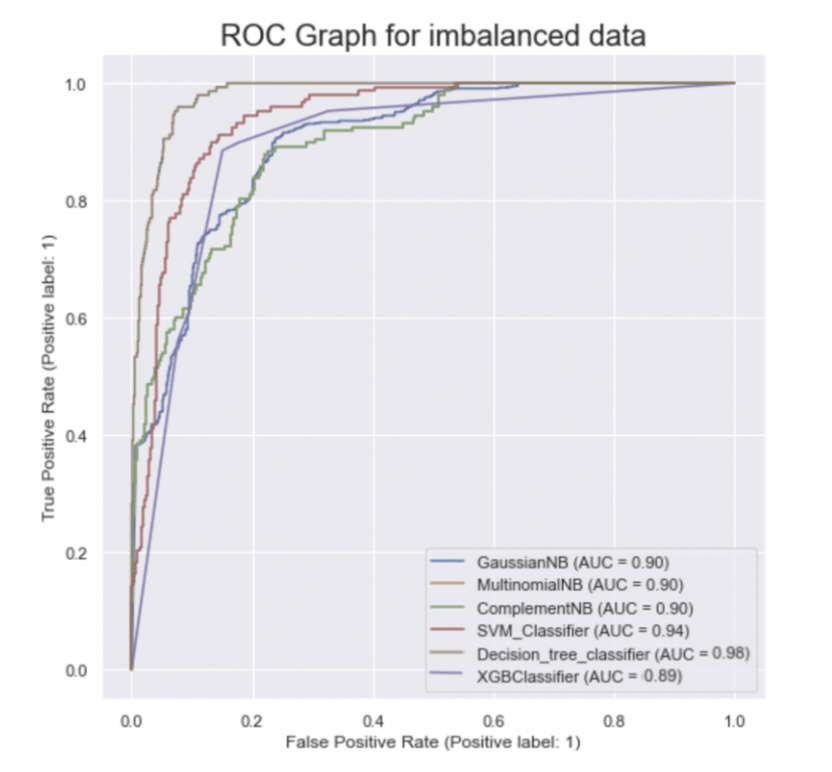
\includegraphics[width=8cm,height=5cm]{Images/Roc_without_sampling_final.png}
    \caption{ROC Curve of Models built on Imbalanced data}
    \label{fig:Roc Curve of Models built on Imbalanced data}
\end{figure}
\\\
\\As we can see from the Fig.20, Decision Tree has highest area under the curve(98 percent).

\begin{figure}[htp]
    \centering
    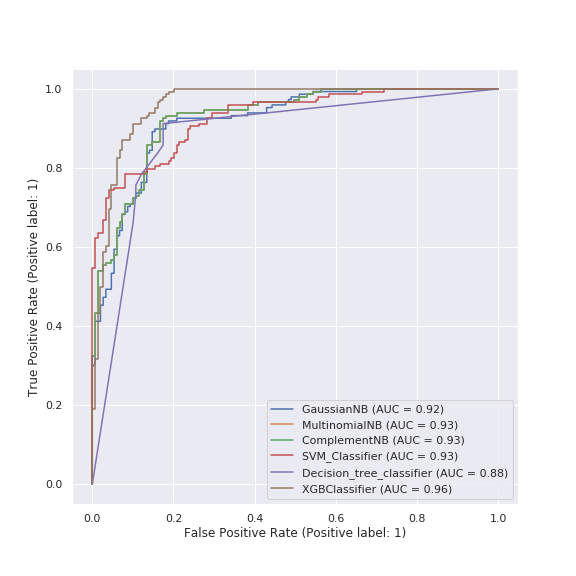
\includegraphics[width=8cm,height=5cm]{Images/Roc_with_undersampling_final.png}
    \caption{Roc Curve of Models built on Undersampling data}
    \label{fig:Roc Curve of Models built on Undersampling data}
\end{figure}
\\\
As we can see from the Fig.21, XGBClassifier has highest area under the curve(98 percent) for balanced data generated using SMOTE technique.

\begin{figure}[htp]
    \centering
    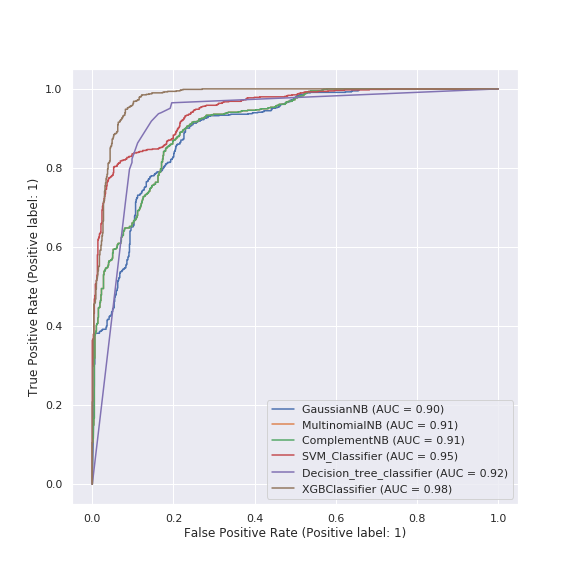
\includegraphics[width=8cm,height=5cm]{Images/Roc_with_SMOTE_final.png}
    \caption{ROC Curve of Models built on SMOTE data}
    \label{fig:Roc Curve of Models built on SMOTE data}
\end{figure}
\\\
\\\
The Fig.22 shows the ROC graph of all types of data discussed, built on various models specified above. 
\\\
\begin{figure}[htp]
    \centering
    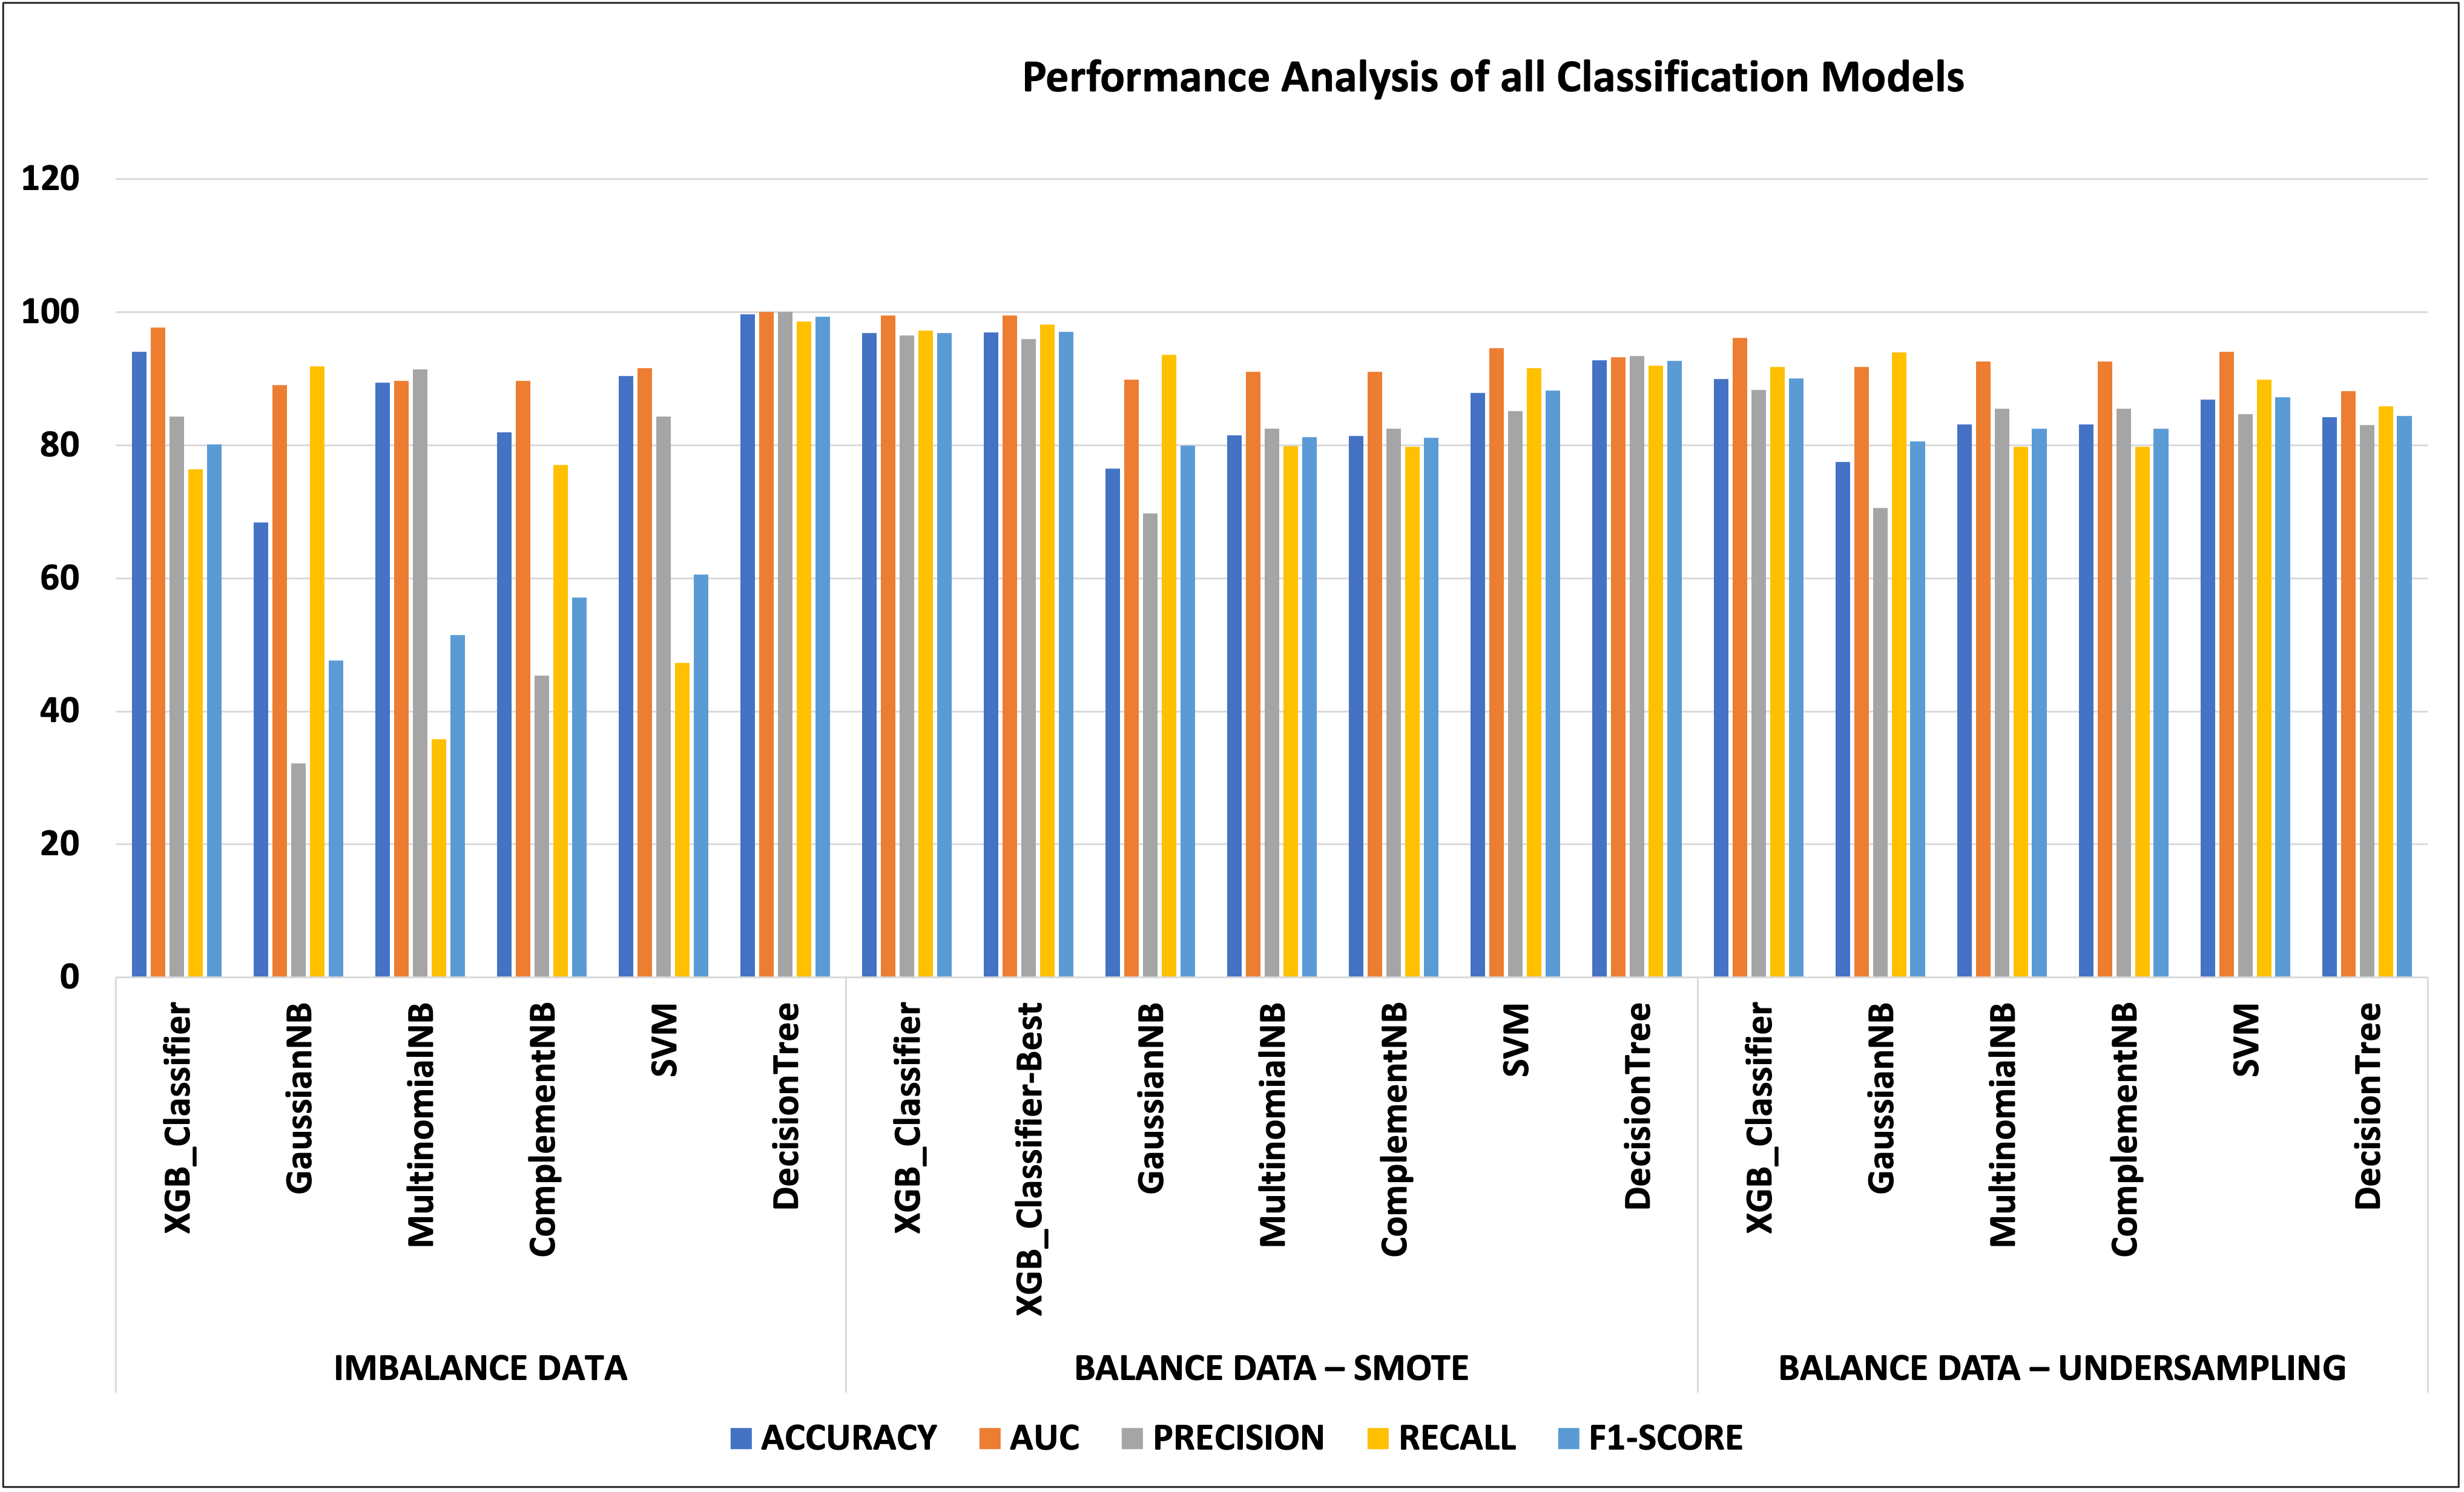
\includegraphics[width=8cm,height=5cm]{Images/performanceAnalysis.png}
    \caption{Performance Analysis of all Classification Models}
    \label{fig:PerformanceAnalysis}
\end{figure}
\\\
\\\
\\\textit{\textbf{Observation:} 
This graph gives us a clear picture of which classifier worked best for the different datasets as it compares metrics like precision,recall,f1-score and AUC for the different classifiers and we infer that decision tree worked better with respect to imbalanced data and XGBoost worked better with respect to balanced data}
\\\
\\\
\section{\textbf{Conclusion}}
In this analysis we experienced four prominent classification techniques using an Iranian telecommunication company dataset. XGBoost significantly outperformed the other classifiers on balanced data while Decision Tress performed the best on imbalanced data set. This study also investigated that complaints and customer status are the major factors that influence customer churn significantly. Based on these factors, we suggest potential approaches that will enable the telecom company reduce the customer attrition rate considerably.
\\\
\\\textbf{Approaches for using customer status as an alarm to churn potential:}
\\a) Monitor the change in customer status as an alarm to churn potential.
\\b) Provide special offers and services to customer with inactive status.
\\c) Identify factors that make the customer status inactive and try to avoid them.

\\\
\\\textbf{Approaches to avoiding customer churn due to dissatisfaction:}
\\a) Conduct direct and indirect polling to determine customer expectations and perceptions about operator services.
\\b) Consider programs for rewarding long-term customers as lucrative assets of the organization.
\\c) Try to improve network coverage.

\\\
\section{\textbf{Limitations and Future Research}}
\\\
Lack of access to different types of data is the main limitation of this study, for example service costs, geographic location, types of service(phone/internet), dependence of customer recount as an important factor of customer churn.  Having multiple service providers data could be very useful for understanding customer retention behavior more thoroughly.  Overcoming these limitations can be done in future research.  Also, customer probable churn time could be considered. Using time series methods can be useful in extracting churn prediction function and calculating customer churn probability in certain time interval.

\\\
\section{\textbf{REFERENCES}}

\\\
\color{teal}
\\\
[1]\textit{\url{ https://analyticsindiamag.com/tips-for-automating-eda-using-pandas-profiling-sweetviz-and-autoviz-in-python/}}
\\\
\\\
[2] \textbf{ Dataset Link:} \\ \textit{ \url{https://tinyurl.com/TelecomCustomerChurnDataset}}
\\\
\\\
[3]  \textit{Ahmed U, Khan A, Khan SH, Basit A, Haq IU, Lee YS (2019) Transfer learning and meta classification based deep churn prediction system for telecom industry.}
\\\
\\\
[4] \textit{Amin A, Anwar S, Adnan A, Nawaz M, Howard N, Qadir J, Hawalah A, Hussain A (2016) Comparing oversampling techniques to handle the class imbalance problem: a customer churn prediction case study. IEEE Access 4:7940–7957}
\\\
\\\
[5] \textit
https://techsee.me/blog/telecom-customer-retention/
\\\
\\\



\end{document}
